\documentclass[a4paper]{article}
\usepackage[breaklinks,colorlinks=true,citecolor=black,linkcolor=black,urlcolor=black,hyperfootnotes=false]{hyperref}
\usepackage{amsmath,amsfonts,amsthm,amssymb}
\usepackage[utf8]{inputenc}
\usepackage{tikz}
\usepackage{pgfplots}
\pgfplotsset{compat=1.17}

\begin{document}

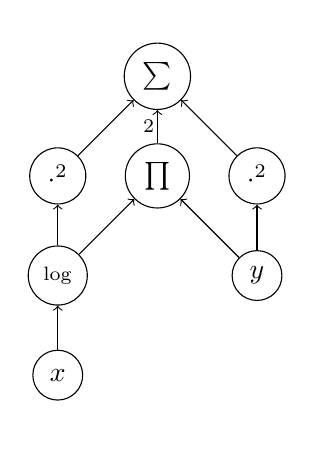
\begin{tikzpicture}[scale=0.6, sibling distance=6em, level distance=6em]
    \tikzstyle{expr} += [shape=circle, draw, align=center, minimum size = 18pt] %

    \node[expr] (plus) {$\sum$}
      child[<-] {
        node[expr] (sqr1) {$\cdot^2$}
        child[<-] {
          node[expr] (log) {\scriptsize $\log$}
          child[<-] {
            node[expr] (x) {$x$}
          }
        }
      }
      child[<-] {
        node[expr] (prod) {$\prod$}
        edge from parent node[left,inner sep=.1em] {\scriptsize 2}
      }
      child[<-] {
        node[expr] (sqr2) {$\cdot^2$}
        child[<-] {
          node[expr] (y) {$y$}
        }
      };

    \draw[<-] (prod) to[out=-135,in=45] (log);
    \draw[<-] (prod) to[out=-45,in=135] (y);

    \node[yshift=+0.5cm] (t3) at (plus) {};

    \node[yshift=-0.5cm]               (t1) at (x) {};
    \node[yshift=-0.5cm]               (t2) at (y) {};
  \end{tikzpicture}

\end{document}